\section{Maximum Flow}
\tikzset{
  in place/.style={
    auto=false,
    fill=white,
    inner sep=2pt,
  },
}
  \tikzstyle{vertex}=[circle,fill=black!25,minimum size=20pt,inner sep=0pt]
  \tikzstyle{source}=[circle,fill=red!25, minimum size = 30pt, inner sep = 0pt]
  \tikzstyle{target}=[circle,fill=blue!25, minimum size = 30pt, inner sep = 0pt]
  \tikzstyle{edge} = [draw,thick,-]
  \tikzstyle{diredge} = [draw,thick,->]
  \tikzstyle{selected diredge} = [draw,thick,->,red]
  \tikzstyle{selected edge} = [draw,thick,-,red]



  % Gerichte Gaphen erzählen
  % Autos pro Zeit
  % Rückkanten idee bei definition
  % def Ford fulkerson
  % Wert von Fluss -> Laufzeit
  % --> f*
  % Math umgebungen
  % wenn du zeit hast \mathcal {0} (T_SDFS)
  \subsection{Motivation}
  \begin{frame}<handout:0>{Beispielaufgabe}
    \setbeamercovered{invisible}
    \begin{block}{Beispielaufgabe}
      \begin{itemize}
        \item Gegeben sei ein Netz mit Städten und Straßen mit einer Kapazität (Autos pro Stunde)
        \pause
        \item Für gewisse Städte A und D sucht man die Anzahl Autos pro Stunde die von A nach D fahren können
      \end{itemize}
    \end{block}
  \end{frame}
    \begin{frame}<handout:0>{Motivation}
  \setbeamercovered{invisible}

    \begin{figure}
        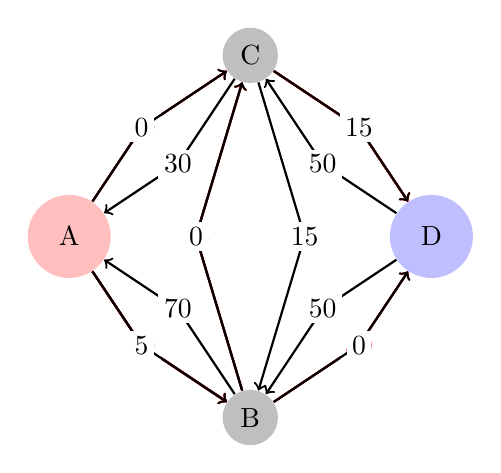
\begin{tikzpicture}[scale=2.3, auto,swap]
        \node[source] (A) at (0, 0) {A};
        \node[vertex] (B) at (1, -1) {B};
        \node[vertex] (C) at (1, 1) {C};
        \node[target] (D) at (2, 0) {D};


    % A - B
    \path[edge]<1> (A) --  (0.4, -0.6);
    \path[diredge]<1> (0.4, -0.6) -- node[pos=0, in place] {70} (B);

    \path[edge]<1-> (B) -- (0.6, -0.4);
    \path[diredge]<1-> (0.6, -0.4) --node[pos=0, in place] {70} (A);

    % A - C
    \path[edge]<1-3> (A) -- (0.4, 0.6);
    \path[diredge]<1-3> (0.4, 0.6) -- node[pos=0, in place] {30} (C);

    \path[edge]<1-> (C) -- (0.6, 0.4);
    \path[diredge]<1-> (0.6, 0.4) -- node[pos=0, in place] {30} (A);

    % C - D
    \path[edge]<1-3> (C) -- (1.6, 0.6);
    \path[diredge]<1-3> (1.6, 0.6) -- node[pos=0, in place] {50} (D);

    \path[edge]<1-> (D) -- (1.4, 0.4);
    \path[diredge]<1-> (1.4, 0.4) -- node[pos=0, in place] {50} (C);

    % B - D
    \path[edge]<1> (B) -- (1.6, -0.6);
    \path[diredge]<1> (1.6, -0.6) -- node[pos=0, in place] {50} (D);

    \path[edge]<1-> (D) -- (1.4, -0.4);
    \path[diredge]<1-> (1.4, -0.4) -- node[pos=0, in place] {50} (B);

    % B - C
    \path[edge]<1-4> (B) -- (0.7,0);
    \path[diredge]<1-4> (0.7, 0) -- node[pos=0, in place] {15} (C);
    \path[diredge]<1-> (1.3,0) -- (B) ;
    \path[edge]<1-> (C) -- node[pos=1, in place] {15} (1.3,0);


    \path[selected edge]<2> (A) --  (0.4, -0.6);
    \path[selected diredge]<2> (0.4, -0.6) -- node[pos=0, in place] {70} (B);

    \path[selected edge]<2> (B) -- (1.6, -0.6);
    \path[selected diredge]<2> (1.6, -0.6) -- node[pos=0, in place] {50} (D);

    \path[edge]<3-4> (A) --  (0.4, -0.6);
    \path[diredge]<3-4> (0.4, -0.6) -- node[pos=0, in place] {20} (B);

    \path[edge]<3-6> (B) -- (1.6, -0.6);
    \path[diredge]<3-6> (1.6, -0.6) -- node[pos=0, in place] {0} (D);

    \path[selected edge]<4> (A) -- (0.4, 0.6);
    \path[selected diredge]<4> (0.4, 0.6) -- node[pos=0, in place] {30} (C);

    \path[selected edge]<4> (C) -- (1.6, 0.6);
    \path[selected diredge]<4> (1.6, 0.6) -- node[pos=0, in place] {50} (D);

    % A - B
    \path[selected edge]<5> (A) --  (0.4, -0.6);
    \path[selected diredge]<5> (0.4, -0.6) -- node[pos=0, in place] {20} (B);

    % A - C
    \path[edge]<5-6> (A) -- (0.4, 0.6);
    \path[diredge]<5-6> (0.4, 0.6) -- node[pos=0, in place] {0} (C);

    % C - D
    \path[selected edge]<5> (C) -- (1.6, 0.6);
    \path[selected diredge]<5> (1.6, 0.6) -- node[pos=0, in place] {20} (D);

    % B - C
    \path[selected edge]<5> (B) -- (0.7,0);
    \path[selected diredge]<5> (0.7, 0) -- node[pos=0, in place] {15} (C);

    \path[edge]<6> (B) -- (0.7,0);
    \path[diredge]<6> (0.7, 0) -- node[pos=0, in place] {0} (C);

    \path[edge]<6> (A) --  (0.4, -0.6);
    \path[diredge]<6> (0.4, -0.6) -- node[pos=0, in place] {5} (B);

    \path[edge]<6> (C) -- (1.6, 0.6);
    \path[diredge]<6> (1.6, 0.6) -- node[pos=0, in place] {15} (D);


    \end{tikzpicture}
  \end{figure}
  \begin{center}
    \pause \pause 50
    \pause \pause  + 30
    \pause  + 15 = 95
  \end{center}


\end{frame}

\subsection{Ford Fulkerson}
\subsubsection{Algorithmus}
\begin{frame}{Ford Fulkerson}
  \setbeamercovered{invisible}
  %\rightarrow
  \begin{block}{Ford Fulkerson}
    \begin{itemize}
      \item $F = 0$
      \pause
      \item Solange ein steigender Pfad p ($s \rightarrow\dots\rightarrow i$ $\rightarrow j\rightarrow\dots\rightarrow t$) von $s$ nach $t$ existiert:
      \pause
      \begin{itemize}
      \item 1. finde minimale Kante $f$ auf dem Pfad
      \pause
      \item 2. Kapazität aller Kanten in Pfadrichtung (z.B. $i\rightarrow j$) um $f$ reduzieren
      \pause
      \item 3. Kapazität aller Kanten gegen Pfadrichtung (z.B. $j\rightarrow i$) um $f$ erhöhen 
      \pause
      \item $F \mathrel{+}= f$;
      \end{itemize}
    \end{itemize}
  \end{block}
\end{frame}
\subsubsection{Rückkante}
\begin{frame}{Rückkante}
  \setbeamercovered{invisible}
  \begin{figure}
    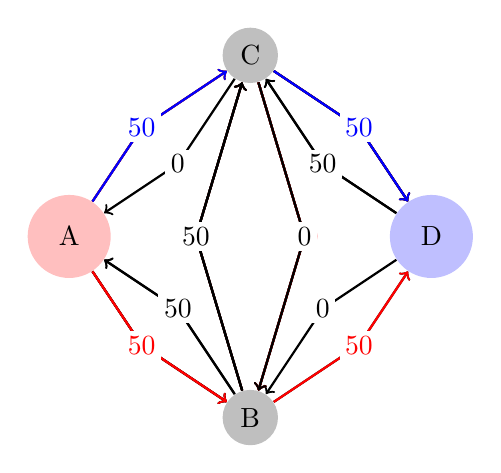
\begin{tikzpicture}[scale=2.3, auto,swap]
    \node[source] (A) at (0, 0) {A};
    \node[vertex] (B) at (1, -1) {B};
    \node[vertex] (C) at (1, 1) {C};
    \node[target] (D) at (2, 0) {D};

    % A - B
    \path[edge]<1 |handout: 1> (A) --  (0.4, -0.6);
    \path[diredge]<1 |handout: 1> (0.4, -0.6) -- node[pos=0, in place] {50} (B);

    \path[edge]<1,2,6 |handout: 1, 2, 5> (B) -- (0.6, -0.4);
    \path[diredge]<1,2,6|handout: 1, 2, 5> (0.6, -0.4) --node[pos=0, in place] {0} (A);

    % A - C
    \path[edge]<1-4|handout: 1-3> (A) -- (0.4, 0.6);
    \path[diredge]<1-4|handout: 1-3> (0.4, 0.6) -- node[pos=0, in place] {50} (C);

    \path[edge]<1- |handout: 1-> (C) -- (0.6, 0.4);
    \path[diredge]<1- |handout: 1-> (0.6, 0.4) -- node[pos=0, in place] {0} (A);

    % C - D
    \path[edge]<1 |handout: 1> (C) -- (1.6, 0.6);
    \path[diredge]<1|handout: 1> (1.6, 0.6) -- node[pos=0, in place] {50} (D);

    \path[edge]<1,2,6|handout: 1, 2, 5> (D) -- (1.4, 0.4);
    \path[diredge]<1,2,6|handout: 1, 2, 5> (1.4, 0.4) -- node[pos=0, in place] {0} (C);

    % B - D
    \path[edge]<1-4|handout: 1-3> (B) -- (1.6, -0.6);
    \path[diredge]<1-4|handout: 1-3> (1.6, -0.6) -- node[pos=0, in place] {50} (D);

    \path[edge]<1- |handout: 1-> (D) -- (1.4, -0.4);
    \path[diredge]<1- |handout: 1-> (1.4, -0.4) -- node[pos=0, in place] {0} (B);

    % B - C
    \path[edge]<1|handout: 1> (B) -- (0.7,0);
    \path[diredge]<1|handout: 1> (0.7, 0) -- node[pos=0, in place] {50} (C);
    \path[diredge]<1,2,6|handout: 1, 2, 5> (1.3,0) -- (B) ;
    \path[edge]<1,2,6|handout: 1, 2, 5> (C) -- node[pos=1, in place] {0} (1.3,0);


    \path[selected edge]<2|handout: 2> (A) --  (0.4, -0.6);
    \path[selected diredge]<2|handout: 2> (0.4, -0.6) -- node[pos=0, in place] {50} (B);

    \path[selected edge]<2|handout: 2> (B) -- (0.7,0);
    \path[selected diredge]<2|handout: 2> (0.7, 0) -- node[pos=0, in place] {50} (C);

    \path[selected edge]<2|handout: 2> (C) -- (1.6, 0.6);
    \path[selected diredge]<2|handout: 2> (1.6, 0.6) -- node[pos=0, in place] {50} (D);

    \path[edge]<3-5|handout: 3-4> (B) -- (0.6, -0.4);
    \path[diredge]<3-5|handout: 3-4> (0.6, -0.4) --node[pos=0, in place] {50} (A);

    \path[diredge]<3|handout: 3> (1.3,0) -- (B) ;
    \path[edge]<3|handout: 3> (C) -- node[pos=1, in place] {50} (1.3,0);

    \path[edge]<3-5|handout: 3-4> (D) -- (1.4, 0.4);
    \path[diredge]<3-5|handout: 3-4> (1.4, 0.4) -- node[pos=0, in place] {50} (C);


    \path[edge]<3-5|handout: 3-4> (A) --  (0.4, -0.6);
    \path[diredge]<3-5|handout: 3-4> (0.4, -0.6) -- node[pos=0, in place] {0} (B);

    \path[edge]<3-5|handout: 3-4> (C) -- (1.6, 0.6);
    \path[diredge]<3-5|handout: 3-4> (1.6, 0.6) -- node[pos=0, in place] {0} (D);

    \path[edge]<3|handout: 3> (B) -- (0.7,0);
    \path[diredge]<3|handout: 3> (0.7, 0) -- node[pos=0, in place] {0} (C);

    \path[edge]<4-5|handout: 3-4> (B) -- (0.7,0);
    \path[diredge]<4-5|handout: 3-4> (0.7, 0) -- node[pos=0, in place] {0} (C);

    \path[diredge]<4|handout: 3> (1.3,0) -- (B) ;
    \path[edge]<4|handout: 3> (C) -- node[pos=1, in place] {50} (1.3,0);

    \path[selected diredge]<5|handout: 4> (1.3,0) -- (B) ;
    \path[selected edge]<5|handout: 4> (C) -- node[pos=1, in place] {50} (1.3,0);

    \path[selected edge]<5|handout: 4> (A) -- (0.4, 0.6);
    \path[selected diredge]<5|handout: 4> (0.4, 0.6) -- node[pos=0, in place] {50} (C);

    \path[selected edge]<5-6|handout: 4-5> (B) -- (1.6, -0.6);
    \path[selected diredge]<5-6|handout: 4-5> (1.6, -0.6) -- node[pos=0, in place] {50} (D);

    \path[edge]<6|handout: 5> (B) -- (0.7,0);
    \path[diredge]<6|handout: 5> (0.7, 0) -- node[pos=0, in place] {50} (C);

    \path[diredge]<6|handout: 5> (1.3,0) -- (B) ;
    \path[edge]<6|handout: 5> (C) -- node[pos=1, in place] {0} (1.3,0);


    \path[selected edge]<6|handout: 5> (A) --  (0.4, -0.6);
    \path[selected diredge]<6|handout: 5> (0.4, -0.6) -- node[pos=0, in place] {50} (B);

    \path[draw, thick, -, blue]<6|handout: 5> (C) -- (1.6, 0.6);
    \path[draw, thick, ->, blue]<6|handout: 5> (1.6, 0.6) -- node[pos=0, in place] {50} (D);

    \path[draw, thick, -, blue]<6|handout: 5> (A) -- (0.4, 0.6);
    \path[draw, thick, ->, blue]<6|handout: 5> (0.4, 0.6) -- node[pos=0, in place] {50} (C);


    \end{tikzpicture}
  \end{figure}
\end{frame}
\subsubsection{Laufzeit}
\begin{frame}{Laufzeit}
  \setbeamercovered{invisible}
  \begin{block}{Laufzeit Ford Fulkerson}
      \begin{itemize}
        \item $\mathcal{O}(F\cdot T_{DFS}) = \mathcal{O}(F\cdot E)$
        \pause
        \item wobei $F$ der Wert des maximalen Flusses ist
        \pause
        \item $\mathcal{O}(F)$ mal Tiefensuche, was in $\mathcal{O}(E)$ läuft, da $E \geq V - 1$
      \end{itemize}
      \pause
      $\Rightarrow$ kann sehr groß werden
  \end{block}
\end{frame}
\begin{frame}{Laufzeit Beispiel}
  \setbeamercovered{invisible}
  \begin{figure}
    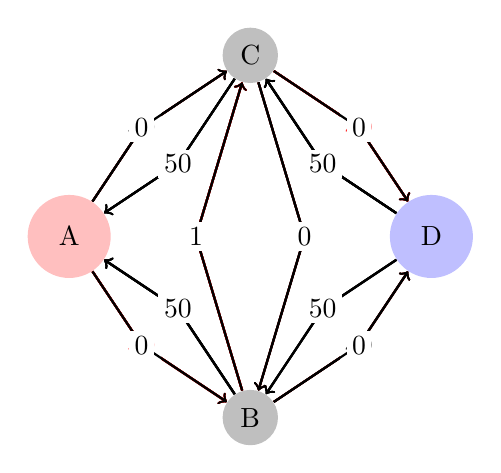
\begin{tikzpicture}[scale=2.3, auto,swap]
    \node[source] (A) at (0, 0) {A};
    \node[vertex] (B) at (1, -1) {B};
    \node[vertex] (C) at (1, 1) {C};
    \node[target] (D) at (2, 0) {D};

    % A - B
    \path[edge]<1|handout: 1> (A) --  (0.4, -0.6);
    \path[diredge]<1|handout: 1> (0.4, -0.6) -- node[pos=0, in place] {50} (B);

    \path[edge]<1-2|handout: 1-2> (B) -- (0.6, -0.4);
    \path[diredge]<1-2|handout: 1-2> (0.6, -0.4) --node[pos=0, in place] {0} (A);

    % A - C
    \path[edge]<1-2|handout: 1-2> (A) -- (0.4, 0.6);
    \path[diredge]<1-2|handout: 1-2> (0.4, 0.6) -- node[pos=0, in place] {50} (C);

    \path[edge]<1-3|handout: 1-3> (C) -- (0.6, 0.4);
    \path[diredge]<1-3|handout: 1-3> (0.6, 0.4) -- node[pos=0, in place] {0} (A);

    % C - D
    \path[edge]<1|handout: 1> (C) -- (1.6, 0.6);
    \path[diredge]<1|handout: 1> (1.6, 0.6) -- node[pos=0, in place] {50} (D);

    \path[edge]<1-2|handout: 1-2> (D) -- (1.4, 0.4);
    \path[diredge]<1-2|handout: 1-2> (1.4, 0.4) -- node[pos=0, in place] {0} (C);

    % B - D
    \path[edge]<1-2|handout: 1-2> (B) -- (1.6, -0.6);
    \path[diredge]<1-2|handout: 1-2> (1.6, -0.6) -- node[pos=0, in place] {50} (D);

    \path[edge]<1-3|handout: 1-3> (D) -- (1.4, -0.4);
    \path[diredge]<1-3|handout: 1-3> (1.4, -0.4) -- node[pos=0, in place] {0} (B);

    % B - C
    \path[edge]<1|handout: 1> (B) -- (0.7,0);
    \path[diredge]<1|handout: 1> (0.7, 0) -- node[pos=0, in place] {1} (C);
    \path[diredge]<1-2|handout: 1-2> (1.3,0) -- (B) ;
    \path[edge]<1-2|handout: 1-2> (C) -- node[pos=1, in place] {0} (1.3,0);

    \path[selected edge]<2|handout: 2> (B) -- (0.7,0);
    \path[selected diredge]<2|handout: 2> (0.7, 0) -- node[pos=0, in place] {1} (C);

    \path[selected edge]<2|handout: 2> (C) -- (1.6, 0.6);
    \path[selected diredge]<2|handout: 2> (1.6, 0.6) -- node[pos=0, in place] {50} (D);

    \path[selected edge]<2|handout: 2> (A) --  (0.4, -0.6);
    \path[selected diredge]<2|handout: 2> (0.4, -0.6) -- node[pos=0, in place] {50} (B);
    % Page 3
    % A - B
    \path[edge]<3|handout: 3> (A) --  (0.4, -0.6);
    \path[diredge]<3|handout: 3> (0.4, -0.6) -- node[pos=0, in place] {49} (B);

    \path[edge]<3-4|handout: 3-4> (B) -- (0.6, -0.4);
    \path[diredge]<3-4|handout: 3-4> (0.6, -0.4) --node[pos=0, in place] {1} (A);

    % A - C
    \path[selected edge]<3|handout: 3> (A) -- (0.4, 0.6);
    \path[selected diredge]<3|handout: 3> (0.4, 0.6) -- node[pos=0, in place] {50} (C);

    % C - D
    \path[edge]<3|handout: 3> (C) -- (1.6, 0.6);
    \path[diredge]<3|handout: 3> (1.6, 0.6) -- node[pos=0, in place] {49} (D);

    \path[edge]<3-4|handout: 3-4> (D) -- (1.4, 0.4);
    \path[diredge]<3-4|handout: 3-4> (1.4, 0.4) -- node[pos=0, in place] {1} (C);

    % B - D
    \path[selected edge]<3|handout: 3> (B) -- (1.6, -0.6);
    \path[selected diredge]<3|handout: 3> (1.6, -0.6) -- node[pos=0, in place] {50} (D);

    % B - C
    \path[edge]<3|handout: 3> (B) -- (0.7,0);
    \path[diredge]<3|handout: 3> (0.7, 0) -- node[pos=0, in place] {0} (C);
    \path[selected diredge]<3|handout: 3> (1.3,0) -- (B) ;
    \path[selected edge]<3|handout: 3> (C) -- node[pos=1, in place] {1} (1.3,0);

    % Page 4
    \path[selected edge]<4|handout: 4> (B) -- (0.7,0);
    \path[selected diredge]<4|handout: 4> (0.7, 0) -- node[pos=0, in place] {1} (C);

    \path[selected edge]<4|handout: 4> (C) -- (1.6, 0.6);
    \path[selected diredge]<4|handout: 4> (1.6, 0.6) -- node[pos=0, in place] {49} (D);

    \path[selected edge]<4|handout: 4> (A) --  (0.4, -0.6);
    \path[selected diredge]<4|handout: 4> (0.4, -0.6) -- node[pos=0, in place] {49} (B);

    \path[diredge]<4|handout: 4> (1.3,0) -- (B) ;
    \path[edge]<4|handout: 4> (C) -- node[pos=1, in place] {0} (1.3,0);

    \path[edge]<4|handout: 4> (B) -- (1.6, -0.6);
    \path[diredge]<4|handout: 4> (1.6, -0.6) -- node[pos=0, in place] {49} (D);

    \path[edge]<4|handout: 4> (D) -- (1.4, -0.4);
    \path[diredge]<4|handout: 4> (1.4, -0.4) -- node[pos=0, in place] {1} (B);

    \path[edge]<4|handout: 4> (D) -- (1.4, 0.4);
    \path[diredge]<4|handout: 4> (1.4, 0.4) -- node[pos=0, in place] {1} (C);

    \path[edge]<4|handout: 4> (A) -- (0.4, 0.6);
    \path[diredge]<4|handout: 4> (0.4, 0.6) -- node[pos=0, in place] {49} (C);

    \path[edge]<4|handout: 4> (C) -- (0.6, 0.4);
    \path[diredge]<4|handout: 4> (0.6, 0.4) -- node[pos=0, in place] {1} (A);

    \path[edge]<4|handout: 4> (B) -- (0.6, -0.4);
    \path[diredge]<4|handout: 4> (0.6, -0.4) --node[pos=0, in place] {1} (A);

    % Page 5

    % A - B
    \path[edge]<5|handout: 5> (A) --  (0.4, -0.6);
    \path[diredge]<5|handout: 5> (0.4, -0.6) -- node[pos=0, in place] {0} (B);

    \path[edge]<5|handout: 5> (B) -- (0.6, -0.4);
    \path[diredge]<5|handout: 5> (0.6, -0.4) --node[pos=0, in place] {50} (A);

    % A - C
    \path[edge]<5|handout: 5> (A) -- (0.4, 0.6);
    \path[diredge]<5|handout: 5> (0.4, 0.6) -- node[pos=0, in place] {0} (C);

    \path[edge]<5|handout: 5> (C) -- (0.6, 0.4);
    \path[diredge]<5|handout: 5> (0.6, 0.4) -- node[pos=0, in place] {50} (A);

    % C - D
    \path[edge]<5|handout: 5> (C) -- (1.6, 0.6);
    \path[diredge]<5|handout: 5> (1.6, 0.6) -- node[pos=0, in place] {0} (D);

    \path[edge]<5|handout: 5> (D) -- (1.4, 0.4);
    \path[diredge]<5|handout: 5> (1.4, 0.4) -- node[pos=0, in place] {50} (C);

    % B - D
    \path[edge]<5|handout: 5> (B) -- (1.6, -0.6);
    \path[diredge]<5|handout: 5> (1.6, -0.6) -- node[pos=0, in place] {0} (D);

    \path[edge]<5|handout: 5> (D) -- (1.4, -0.4);
    \path[diredge]<5|handout: 5> (1.4, -0.4) -- node[pos=0, in place] {50} (B);

    % B - C
    \path[edge]<5|handout: 5> (B) -- (0.7,0);
    \path[diredge]<5|handout: 5> (0.7, 0) -- node[pos=0, in place] {1} (C);
    \path[diredge]<5|handout: 5> (1.3,0) -- (B) ;
    \path[edge]<5|handout: 5> (C) -- node[pos=1, in place] {0} (1.3,0);

    \end{tikzpicture}
  \end{figure}


\end{frame}
\subsection{Edmond Karp}
\begin{frame}{Edmond Karp}
  \setbeamercovered{invisible}
  \begin{block}{Unterschied zu Ford Fulkerson}
    \begin{itemize}
      \item Breitensuche statt Tiefensuche
      \pause
      \item Laufzeit $\mathcal{O}(VE^2)$
      \pause
      \item $\mathcal{O}(VE)$ mal Breitensuche, was in $\mathcal{O}(E)$ läuft
    \end{itemize}
  \end{block}
\end{frame}